%!TEX root = ../CombinatoricsNotes.tex

\section{Algebraic methods}
% \marginnote{Lecture X: Wednesday, April 6, 2016.}
\lect{2}{6}

\subsection{Combinatorial Nullstellensatz (\cite{AlonTarsi89})}
\newthought{For background} we will first consider the following result about zeros of multivariate polynomials.  
\begin{theorem*}[Hilbert Nullstellensatz (\cite{HilbertNull})]
Let $\F$ be an algebraically closed field. Let $g_1,g_2,\dotsc,g_m \in \F[x_1,x_2,\dotsc,x_n]$ be polynomials of $n$ variables over $\F$. Suppose $f\in \F[x_1,\dotsc,x_n]$ is such that $f=0$ whenever $g_1=g_2=\dotsm = g_m = 0$.
\marginnote{In one variable: $g = (x-a_1)\cdot (x-a_2)\dotsm (x-a_z)$. Assume all roots are distinct. Then $f=0$ at zeros of $g$ iff $f = gh$ for some $h$. If not all roots are distinct, then $f=0$ at zeros of $g$ iff $f^k  =gh$ for some $k\in \N$.}
Then there exists $n\in \N$ and polynomials $h_1,\dotsc,h_m \in \F[x_1,\dotsc,x_n]$ such that $f^n = h_1 g_1 + h_2 g_2 + \dotsm + h_m g_m$.
\end{theorem*}



\newthought{Let us proceed} to \defn{Combinatorial Nullenstellensatz}.
Recall the degree of a multivariable monomial is the sum of degrees in each variable (e.g. $\deg (x_1^2 x_2^3) = 5$), and the degree of a polynomial is as usual the maximum degree of its monomials.
\begin{theorem} \label{thm:comb_nullstell}
Let $\F$ be a field, $S_1,S_2,\dotsc,S_n\subset \F$, 
\[
g_i = \prod_{s\in S_i}(x_i - s)
\]
for $i=1,2,\dotsc, n$.
If $f\in \F[x_1,\dotsc,x_n]$ such that $f$ vanishes on all common zeros of $g_1,g_2,\dotsc,g_n$ (i.e., $f(x_1,\dotsc,x_n) = 0$ if $x_i\in S_i$ for all $i$), then there exist polynomials $h_1,h_2,\dotsc,h_n\in \F[x_1,\dotsc,x_n]$ with $\deg h_i \leq \deg f - \deg g_i$ and $f = h_1g_1 + h_2g_2 + \dotsm + h_n g_n$.
\end{theorem}
\begin{remark}
The $g_i$ are monic, single variable, with no double roots. This is very restrictive compared to Hilbert's Nullstellensatz, but we do obtain a stronger conclusion.
\end{remark}
\marginnote{The degree bound in \cref{thm:comb_nullstell}  means that each $h_ig_i$ has degree at most that of $f$.}
Given a multivariable polynomial $p(x_1,\dotsc,x_n)$, let us denote $\deg_{x_i} p$ as the ``degree of $p$ over $x_i$'', i.e. the degree of $p$ when considered as a polynomial in the variable $x_i$ only, treating $x_1,\dotsc,x_{i-1},x_{i+1},\dotsc,x_n$ as constants. To prove \cref{thm:comb_nullstell}, we'll need the following lemma.
% \marginnote{}
\begin{lemma} \label{lem:comb_null_p_vanish}
Let $P\in \F[x_1,\dotsc,x_n]$ with $\deg_{x_i} P \leq t_i$ for $i=1,\dotsc,n$. Let $S_1,\dotsc, S_n \subset \F$ , $|S_i|\geq t_i+1$ for $i\in[n]$. If $P (x_1,\dotsc,x_n) = 0$ when  $x_i\in S_i$ for each $i\in [n]$, then $P \equiv 0$.
\end{lemma}
\begin{proof}[Proof by induction on $n$.]
Base case $(n=1)$: a degree $t$ polynomial has at most $t$ roots.
Induction step: we write
\begin{fullwidth}
\begin{align*}	
P(x_1,\dotsc,x_n) &= P_{t_n}(x_1,\dotsc,x_{n-1}) x_n^{t_n} + \dotsm + P_1 (x_1,\dotsc,x_{n-1}) x_n + P_0 (x_1,\dotsc,x_{n-1}) \\
&= \sum_{i=1}^{t_n} P_{t_i}(x_1,\dotsc,x_{n-1}) x_n^i.
\end{align*}
\end{fullwidth}
for some polynomials $P_{t_n},\dotsc,P_0$ in variables $x_1,\dotsc,x_{n-1}$. \marginnote{I.e., the $P_{t_i}$ are the coefficients of $x_n^i$, and do not depend on $x_n$.}
Now, fix $x_1\in S_1$, \ldots, $x_{n-1} \in S_{n-1}$. Then $P(x_1,\dotsc,x_n)$ becomes a one-variable polynomial in $x_n$ of degree at most $t_n$ with at least $t_n+1$ roots (one for each $x_n \in S_n$). So by the base case, each $P_i(x_1,\dotsc,x_{n-1}) = 0$ for $i\in[t_n]$. Since we chose $x_1\in S_1$, \ldots, $x_{n-1}\in S_{n-1}$ arbitrarily, by the induction hypothesis, $P_i \equiv 0$. Hence $P\equiv 0$.
\end{proof}
We may proceed to prove the theorem.
\begin{proof}[Proof of \cref{thm:comb_nullstell}]

Let $t_i = |S_i| - 1$.  For $i\in [n]$, we write
\[
g_i = x_i^{t_i+1} - \sum_{j=0}^{t_i} a_{ij} x_i^j
\]
for some coefficients $a_{ij}$.
Given a polynomial $f$ in variables $x_1,\dotsc, x_n$, we ``divide with remainder'' by each $g_i$, yielding
\[
f = \left( \sum_{i=1}^n h_i g_i \right) + P.
\]
with $\deg(h_i) \leq \deg(f) - \deg (g_i)$ and $\deg_{x_i} (P)\leq t_i$. Now, if $f$ vanishes when all $x_i\in S_i$, then $P$ does too, so \cref{lem:comb_null_p_vanish} we have $P\equiv 0$, giving the result.
\end{proof}

We may reformulate this result into a perhaps more helpful form.

\begin{theorem}[Combinatorial Nullstellensatz] \label{thm:comb_nullstell_nonzero}
Let $\F$ be a field, $f\in \F[x_1,\dotsc,x_n]$, $\deg(f) = t_1 + t_2 + \dotsm + t_n$ and the coefficient of $x_1^{t_1}x_2^{t_2}\dotsm x_n^{t_n}$ in $f$  non-zero. Let $S_1,S_2,\dotsc,S_n\subset \F$ with $|S_i| \geq t_i+1$. Then there exists $s_1\in S_1$, $s_2\in S_2$,\ldots, $s_n \in S_n$ such that $f(s_1,s_2,\dotsc,s_n) \neq 0$.
\end{theorem}
\begin{proof}	
Suppose not. Then $f$ vanishes whenever $x_i \in S_i$, so by \cref{thm:comb_nullstell}, there exist polynomials $h_1,\dotsc,h_n$ with $\deg(h_i) \leq \deg (f) - |S_i| \leq \deg (f) - t_i -1$ such that
\[
f = \sum_{i=1}^n h_i g_i
\]
where $g_i = \prod_{s\in S_i}(x_i-s)$. Then the monomial $x_1^{t_1}x_2^{t_2}\dotsm x_n^{t_n}$ must appear with non-zero coefficient in some $h_ig_i$. Since $\deg f \geq \deg h_i + \deg g_i$, this term must be obtained by multiplying a  monomial in $h_i$ by the highest degree monomial in $g_i$, namely $x_i^{|S_i|}$. Since $|S_i| > t_i$, this is a contradiction.
\end{proof}


\begin{theorem*}[Cauchy-Davenport theorem]
Let $A,B \subset \Z/ p\Z =: \Z_p$ for $p$ prime. Then $|A+B| \geq \min\{ p, |A|+|B|-1\}$.
\end{theorem*}
% \begin{remark}
% \missing{put in ref to old C-D thoerem}
% \end{remark}
\begin{proof}	
Suppose $|A|+|B| \leq p+1$ without loss of generality\sidenote{by throwing away elements of $A$ and $B$. If the minimum $m$ is acheived by $p$, we throw away elements until $|A|+|B|-1 = p = m$. Then we show that the now-smaller $|A+B|$ has $|A+B| \geq m$. Then the original $|A+B|$ must be at least $m$ as well.}. Suppose, for contradiction, that $|A+B| \leq |A|+|B|- 2$. Then select $C\supseteq A+B$ such that $|C| = |A| + |B| - 2$.

Let $a= |A|$ and $b=|B|$. Set $f(x,y) = \prod_{c\in C} (x+y-c)$. Then 
\[
\deg f = |C| = a+b-2 = \overbrace{(a-1)}^{t_1} + \overbrace{(b-1)}^{t_2}
\]
The coefficient of $x_1^{t_1}x_2^{t_2}$ in $f$ is ${a+b-2\choose a-1}$. Note since $a+b-2 \leq p+1-2 = p-1 < p$ so the binomial coefficient is not zero. Set $S_1= A$, $S_2=B$. By \cref{thm:comb_nullstell_nonzero}, there exists $s_1\in A$, $s_2\in B$ such that $f(s_1,s_2) \neq 0$. Then $s_1+s_2\not\in C$ which is a contradiction.
\end{proof}

Let us consider a conjecture by \cite{ErdosHeilbronn}, proven in 1994. 
\begin{theorem}[\cite{SilvaHamidoune1994}]
Let $A,B\subset \Z_p$, with $A\oplus B = \{a+b: a\in A, b\in B, a\neq b\}$. Then
\[
|A\oplus B| \geq \min \{p, |A| +|B|-2 \}
\]
if $|A|\neq |B|$.
\end{theorem}
\begin{remark}
The assumption $|A|\neq|B|$ is necessary. Say $A= \{0,1,\dotsc,k\}$ with $k< p/2$, then $|A| = k+1$ and
\[
A\oplus A = \{1,2,\dotsc,2k-1 \}
\]
so $|A\oplus A| = 2k-1 = 2|A|-3$.
\end{remark}
\begin{proof}	
Let $a=|A|$, $b=|B|$. WLOG, assume $a+b\leq p+2$. Suppose for a contradiction that  there exists $C \supset A\oplus B$ such that $|C| = a+b-3$. Let 
\[
f(x,y) = (x-y)\prod_{c\in C} (x+y-c).
\]
Then $\deg f = |C|+1 = a+b-2 = (a-1) + (b-1)$. Assume for now that the coefficient of $x^{a-1}y^{b-1}$ is non-zero. Then by \cref{thm:comb_nullstell_nonzero} there exists $s_1\in A$, $s_2\in B$ such that $f(s_1,s_2) \neq 0$. But then $s_1\neq s_2$ and $s_1+s_2\not \in C$. This is a contradiction.

It remains to find the coefficient of $x^{a-1}y^{b-1}$ in $f(x,y)$. The coefficient must be the same as in the polynomial $(x-y)(x+y)^{a+b-3}$. We use binomial expansion and only keep the terms of the right degree: $(x-y) (\alpha_1 x^{a-2}y^{b-1} +  \alpha_2  x^{a-1} y^{b-2})$. Then the coefficient is
\[
\alpha_1 - \alpha_2 = {a+b-3 \choose a-2} - {a+b-3 \choose a-1} \neq 0 \pmod{p}
\]
if and only if
\[
\frac{(a+b-3)!}{(a-2)!(b-1)!} \neq \frac{(a+b-3)!}{(a-1)!(b-2)!} \pmod{p}
\]
which we may simplify to obtain
\[
a-1 \neq b-1 \pmod{p}.\qedhere
\]
\end{proof}


\paragraph{$n$-dimensional hypercube}
$Q_n:=\{0,1\}^n = \{(x_1,\dotsc,x_n) \in \R^n: x_i \in \{0,1\}\}$. $2^n$ points. See \cref{fig:cube} for $Q_3$.
We'd like to cover $Q_n$ by affine hyperplanes; this can be done with $2$: one on top and one on bottom. 
Suppose we'd like to cover exactly all verticies except the origin.



\begin{marginfigure}
\begin{center}
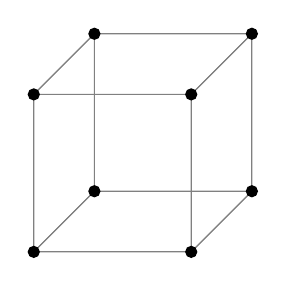
\begin{tikzpicture}
\newcommand{\Depth}{2}
\newcommand{\Height}{2}
\newcommand{\Width}{2}
\def\radius{2pt}
\coordinate (O) at (0,0,0);
\coordinate (A) at (0,\Width,0);
\coordinate (B) at (0,\Width,\Height);
\coordinate (C) at (0,0,\Height);
\coordinate (D) at (\Depth,0,0);
\coordinate (E) at (\Depth,\Width,0);
\coordinate (F) at (\Depth,\Width,\Height);
\coordinate (G) at (\Depth,0,\Height);



\draw[black!50] (O) -- (C) -- (G) -- (D) -- cycle;% Bottom Face
\draw[black!50] (O) -- (A) -- (E) -- (D) -- cycle;% Back Face
\draw[black!50] (O) -- (A) -- (B) -- (C) -- cycle;% Left Face
\draw[black!50] (D) -- (E) -- (F) -- (G) -- cycle;% Right Face
\draw[black!50] (C) -- (B) -- (F) -- (G) -- cycle;% Front Face
\draw[black!50] (A) -- (B) -- (F) -- (E) -- cycle;% Top Face

\filldraw (O) circle(\radius);
\filldraw (A) circle(\radius);
\filldraw (B) circle(\radius);
\filldraw (C) circle(\radius);
\filldraw (D) circle(\radius);
\filldraw (E) circle(\radius);
\filldraw (F) circle(\radius);
\filldraw (G) circle(\radius);

%% Following is for debugging purposes so you can see where the points are
%% These are last so that they show up on top
%\foreach \xy in {O, A, B, C, D, E, F, G}{
%    \node at (\xy) {\xy};
%}
\end{tikzpicture}
\end{center}
\caption{The cube $Q_3$.}\label{fig:cube}
\end{marginfigure}
\begin{theorem}[\cite{AlonFuredi1993}]
Let $H_1,H_2,\dotsc,H_m$ be affine hyperplanes in $\R^n$ with cover exactly $2^n-1$ vertices of the $n$-dimensinal hypercube $Q_n$. Then $m\geq n$.
\end{theorem}
\lect{4}{11}
\begin{proof}	
Let $H_i = \{x: \braket{a_i,x} = b_i\}$ for some $a_i = (a_{i_1},\dotsc,a_{i_n})\in \R^n$ and $b_i\in \R$. That is, if $x=(x_1,\dotsc,x_n)\in H_i$,
\[
a_{i_1}x_1 + a_{i_2}x_2 + \dotsm + a_{i_n}x_n = b_i.
\]
Assume for contradiction that $m<n$, and $H_1,\dotsc,H_m$ do not cover the vertex $(0,0,\dotsc,0)$\marginnote{The vertex $\vec 0$ was chosen without loss of generality, of course.}, but cover every $x = (x_1,\dotsc,x_n)$ for $x_i\in \{0,1\}$ with not all $x_i = 0$. Define
\[
h(x_1,\dotsc,x_n) = \prod_{i=1}^m (\braket{a_i,x} - b_i).
\]
Then by assumption, $h=0$ for every vertex of $Q_n$ except $0$.\marginnote{Note then $h(0,\dotsc,0) = \prod_{i=1}^m (-b_i) \neq 0$.} Using the language of \cref{thm:comb_nullstell_nonzero}, set $S_i = \{0,1\}$, $t_i=1$. We want to choose a polynomial $f$ with $\deg(f)=n$, the coefficient of $x_1\dotsm x_n$ non-zero, and $f(x)=0$ for every vertex of $Q_n$. Our polynomial $h$ will not suffice because $\deg h =m < n$ and in particular the coefficient of $x_1\dotsm x_n$ is zero. Instead, set
\[
f(x_1,\dotsc,x_n) := (-1)^{m+n+1}  \prod_{i=1}^m b_i \prod_{i=1}^n (x_i - 1) + h(x_1,\dotsc,x_n).
\]
Then $\deg f = n$ and the coefficient of $x_1\dotsm x_n$ is $(-1)^{m+n+1} \prod_{i=1}^m b_i \neq 0$.
\Cref{thm:comb_nullstell_nonzero} then yields some $x_1\in S_1$, \ldots, $x_n \in S_n$ such that $f(x_1,\dotsc,x_n)\neq 0$. Since  if $x_i \in \{0,1\}$ not all zero, the first term of $f$ vanishes (because at least one $x_i=1$), and $h$ vanishes by assumption, we must have $x_i\equiv 0$. But then
\[
0 \neq f(0,\dotsc,0) = -(-1)^{m}  \prod_{i=1}^m b_i + h(0,\dotsc,0) = -(-1)^m \prod_{i=1}^m b_i + (-1)^m \prod_{i=1}^m b_i
\]which is a contradiction.
\end{proof}

% \marginnote{Lecture X,  Monday April 11, 2016}

%Lemma 10.6
\begin{lemma} \label{lem:permanent}
Let $A$ be an $n\times n$ matrix over a field $\field$. Suppose $\per(A)\neq 0$.
% , where  if $A = (a_{ij})$,
\marginnote{
The \emph{permanent} of $A$, if $A = (a_{ij})$, is
\[
\per (A) = \sum_{\pi \in S_n} \prod_{i=1}^n a_{i \pi(i)},
\]
i.e. is the determinant without the signs. For example, $\per \begin{pmatrix}
a & b\\ c & d
\end{pmatrix} = ad+bc$. Unlike the determinant, it is not known to be efficiently computable.}
Let $S_1,S_2,\dotsc,S_n \subset \F$, $|S_i| = 2$ for every $i$. Let $b\in \F^n$. Then there exist $x_1\in S_1$, $x_2\in S_2$, \ldots, $x_n\in S_n$ such that if $x = (x_1,\dotsc,x_n)$, then $(Ax)_j \neq b_j$ for every $j=1,\dotsc, n$.
\end{lemma}
\begin{proof}	
Let $f(x_1,\dotsc,x_n) = \prod_{i=1}^n (a_{i1}x_1 + a_{i2}x_2 + \dotsm + a_{in}x_n - b_i)$. By \cref{thm:comb_nullstell_nonzero}, we can find $x_i\in S_i$ such that $f(x_1,\dotsc,x_n)\neq 0$, as desired, if the coefficient of $x_1,\dotsc,x_n$ in $f$ is non-zero. But this coefficient is exactly the permanent of $A$.
\end{proof}

Let $a_1,a_2,\dotsc,a_k$ be integers. We'd like to find nonempty $S\subset[k]$ such that $\sum_{i\in S} a_i$ is divisible by $n$. How large must $k$ be (as a function of $n$)?

One needs at least $n$, as shown by taking $a_i= 1$ for every $i$.

In fact, $k=n$ suffices. Consider $\sigma_i = \sum_{j=1}^i a_j$ for $i=1,\dotsc,n$, i.e., $\sigma_1 = a_1$, $\sigma_2 = a_1 + a_2$, etc. If $\sigma_i \neq 0 \pmod{n}$ for every $n$, then there must exist $i,j$ such that $\sigma_i = \sigma_j \pmod{n}$. But then $\{i+1,\dotsc,j\}$ is the required set.\marginnote{If $\sigma_i = 0 \pmod{n}$ for some $i$, $\{1,2,\dotsc,i\}$ suffices. }


Now, let $a_1,\dotsc,a_k$ be integers. We'd like to find $S\subset [k]$ with $|S| = m$ such that $n$ divides $\sum_{i\in S} a_i$. If $m< n$, we can never guarantee the existence of $S$, as the example $a_i\equiv 1$ shows. In fact, we need at least $m$ divisible by $n$. Let us take $m=n$. 

Suppose $n=2$. How many integers must we have such that two of them sum to an even number? $k=3$; then there is always at least two evens or two odds.

Consider $n=3$. We note $\{0,0,1,1\}$ has no 3 numbers summing to a number divisible by 3. But $k=5$ suffices.

In general, $k=2n-1$. For $2n-2$, we may take $n-1$ $0$'s and $n-1$ $1$'s as a counterexample.

\begin{theorem}[\cite{ErdosGinzburgZiv1961}]
Let $a_1,a_2,\dotsc,a_{2n-1}\in \Z$ be integers. Then there exists $S\subset [2n-1]$ with $|S| = n$ such that $\sum_{i\in S} a_i$ is divisible by $n$.
\end{theorem}
\begin{proof}	
Assume that $n=p$ is prime. We may reduce modulo $p$ to assume $0\leq a_i \leq p-1$ and an ordering $a_1\leq a_2 \leq \dotsm \leq a_{2p-1}$. Let $S_i = \{a_i,a_{i+p-1}\}$ for $i=1,\dotsc,p-1$. Let $A$ be the all $1$'s matrix: $a_{ij} = 1$ for all $1\leq i,j\leq p-1$.

Let $\{b_1,\dotsc,b_{p-1}\}$ be all elements of $\Z_p$ except $-a_{2p-1}$.

\begin{example}
$p=3$, $a_1,a_2,\dotsc,a_5$. $S_1 = \{a_1,a_3\}$, $S_2 = \{a_2,a_4\}$. Suppose $a_5=2$. Then $\{b_1,b_2\} = \{0,2\}$.
\[
\begin{pmatrix}
1 & 1\\
1 & 1
\end{pmatrix} \begin{pmatrix}
a_1 \text{ or } a_3 \\ a_2 \text{ or } a_4
\end{pmatrix} \neq \begin{pmatrix}
0 \\ 2
\end{pmatrix}
\]
where the inequality in fact occurs componentwise.
\end{example}


Suppose there exists $s_1\in S_1$, \ldots, $s_{p-1} \in S_{p-1}$ such that for $s = (s_1,\dotsc,s_{p-1})$, 
\[
As \neq \begin{pmatrix}
b_1 \\ \vdots \\ b_{p-1}
\end{pmatrix}
\]
where the inequality occurs for each coordinate. Equivalently, $s_1 + s_2 + \dotsm + s_{p-1} = - a_{2p-1} \pmod{p}$. That is, $s_1 + \dotsm +  s_{p-1} + a_{2p-1} =  0 \pmod{p}$.

We may find such $s_1,\dotsc,s_{p-1}$ using \cref{lem:permanent}, using that
\[
\per \begin{pmatrix}
1 & \dotsm & 1\\
\vdots & & \vdots \\
1 & \dotsm & 1
\end{pmatrix} = (p-1)! \neq 0 \pmod{p}.
\]
However, we still need to check the condition $|S_i| = 2$ for each $S_i$. If for some $i$ we have $|S_i|=1$, then, $a_i = a_{i+p-1}$. In such a case, by our ordering, $a_i = a_{i+1} = \dotsm = a_{i+p-1}$,  hence
\[
\sum_{j=1}^{i + p-1} a_j = 0 \pmod{p}
\]
as desired.
The composite case will be left as an exercise by induction.
\end{proof}


\subsection{Kakeya needle problem (\cite{Kakeya})}
What is the minimum area of a region in the plane in which one can continuously rotate by 360\textdegree  a needle of length 1? \Cref{fig:needle_circ_tri} shows two attempts.
In fact, the answer is zero.
\begin{marginfigure}
\hfill
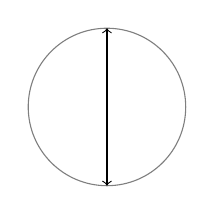
\begin{tikzpicture}[scale=2]
\draw[opacity=.5] (0,0) circle (0.5);
\draw[<->] (0,-.5) -- (0,.5);
\end{tikzpicture}
\hfill
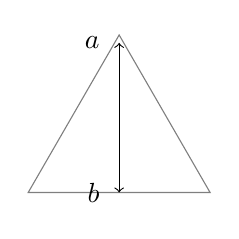
\begin{tikzpicture}[scale=2]
\def\x{2/1.732}
\coordinate (a) at (0,0);
\coordinate (b) at (\x/2,1);
\coordinate (c) at (\x,0);
\draw[opacity=.5] (a)--(b) -- (c) -- cycle;
\draw[<->] (\x/2,0) node[label=left:$b$]{} -- (\x/2,.95)node[label=left:$a$]{};
\end{tikzpicture}
\hfill
\caption{Left: we may simply rotate our needle of length about its middle, using a circle area of $\pi/4$. Right: we could rotate our needle by pulling end $b$ to the bottom left corner of the triangle, then end $a$ down the right side of the triangle. Then we could pull $b$ up the left side of the triangle, and finally $a$ to the middle, therby completing the rotation. This uses an equilateral triangle of altitude $1$, which then has area $\frac{1}{\sqrt{3}}$.} \label{fig:needle_circ_tri}
\end{marginfigure}

Let us try to restate this in terms of finite fields. First, we have the equivalent\sidenote{It turns out these are equivalent, by adding regions of area zero connecting the segments in each direction.} question: What is the minimum area of a region in the plane in which contains a segment of length 1 in every direction?

Now, we have the finite field Kakeya problem: What is the minimum $|E|$ such that $E\subset \field^d$ and $E$ contains a \emph{line} in every direction. That is, for every $v\in \field^d\setminus\{0\}$ there exists $x_v$ such that $x_v + tv\in E$ for every $t\in \field$.
In particular, does there exist $c_d>0$ (depending on $d$ but not $\field$) such that
\[
|E| \geq c_d |\field|^d
\]
for all finite fields $\field$?
% This is in a dual sense to Combinatorial Nullenstallsatz, which says roughly that if $f$ is a low-degree polynomial is cannot vanish everywhere on a set of a certain structure. Here, we will show that with a set of a different st
\begin{lemma}\label{lem10p8:polynomial_vanishes_on_E}
Let $E\subset \F^d$ such that $|E|< {k+d \choose k}$. Then there exists non-zero polynomial $f$ of $d$ variables such  $f(x)=0$ for every $x\in E$, and $\deg f \leq k$. 
\end{lemma}
\begin{proof}	
Let $V$ be the vector space of polynomials in $d$ variables over $\F$ of degree at most $k$. Then $\dim V$ is the number of monomials $x_1^{k_1}x_2^{k_2}\dotsm x_d^{k_d}$ such that $k_1+k_2+\dotsc+k_d \leq k$. This is the same as the number of decompositions $k_1 + k_2 + \dotsm + k_d + k_{d+1} = k$ such that $k_i\geq 0$, $k_i \in \Z$. This is ${k+d \choose k}$ as follows:
 if we write $k$ stars
\[
\star \star \star \star \star \dotsm \star\]
then our task is to put $d$ bars between the stars and thus partition the elements into $k_1,k_2,\dotsc,k_{d+1}$
\[
 \operatorname*{\star}_{k_1}|\operatorname*{\star \star \star}_{k_2} | \star \dotsm \star
\]
sowe must choose $k$ stars from the $k+d$ total number of symbols.

Let $E = \{x_1,\dotsc,x_m\}\subset\field^d$. For $p\in V$, the map
\[
p\mapsto ( p(x^1),p(x^2),\dotsc,p(x^m))
\]
is a linear map from $V$ to $|E|$-dimensional space.
If $\dim(V) > |E|$, then there exists $p\in V$, $p\neq 0$ such that $p$ is mapped to zero, i.e. $p$ is zero everywhere on $E$.
\end{proof}
\lect{4}{13}
% \marginnote{Lecture X: Wednesday, April 13, 2016}
Now, given $\field$ a finite field, we will say $E\subset \field^d$ is a \defn{Kakeya set} if for every $v\in \field^d \setminus \{0\}$ there exists $x\in \field^d$ such that $x+tv \in E$ for every $t$.
\begin{lemma}
If $E\subset \field^d$ is Kakeya, then there exists no $p\in \field[x_1,\dotsc,x_d]$, $p\neq 0$, $\deg p\leq |F| - 1$ such that $p(x) = 0$ for every $x\in E$.
\end{lemma}
\begin{proof}	
Suppose such $p$ exists. Then
\[
p(x) = p_k(x) + p_{k-1}(x) + \dotsm + p_0(x)
\]
where $p_i(x)$ is homogenous polynomial of degree $i$ and $p_k(x)$ not identically $0$ ($\deg p = k$).
By definition, for every $v\in \field^d$ there exists $x$ such that $p(x+tv) =0$ for every $t\in \field$. Fix $x$ and $v$, $p(x+tv)$ is a polynomial in $t$ of degree $\leq |F| - 1$. If $x= ( x_1,\dotsc,x_d)$ and $v = ( v_1,\dotsc,v_d)$, then $x+tv = (x_1+tv_1,\dotsc,x_d+ tv_d)$. The coefficient of $t^k$ in $p$ is $p_k(v)$.

On the other hand, $p$ has $|F|$ roots so $p$ is identically zero as a polynomial in $t$. In particular, $p_k(v) = 0$. But this is true for every $v$, contradicting the assumption that $p_k(v) $ is not identically zero.
\end{proof}

\begin{corollary}[\cite{dvir2009size}]
If $E\subset \field^d$ is Kakeya, then
\[
|E| \geq {|F| - 1 + d \choose d} = \frac{|\field|^d}{d!} + o(|\field|^d).
\]
\end{corollary}



\subsection{Shannon capacity (\cite{shannonGraph})}
We are transmitting messages in alphabet $V$ over a noisy channel. Some symbols can be confused with each other during transmission.

Let $G$ be a graph with vertex set $V$ with a pair of symbols joined by an edge if they can be confounded. 

\begin{example}
$V = \{a,b,d,p,q\}$.

\begin{figure}
\begin{center}
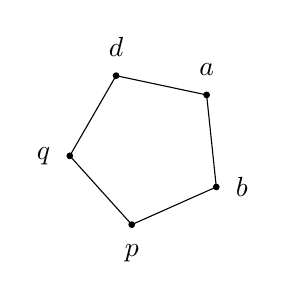
\begin{tikzpicture}%[color=DarkBlue]
\def\n{5}
\def\radius{1}
\def\rotation{-30}
\def\circrad{1pt}
\def\deg{360/\n}
\pgfmathsetmacro\nminusone{\n-1}

% \foreach \x in {1,...,\n}
% {
	\def\x{1}
	\pgfmathsetmacro\myangle{\x*\deg+\rotation};
	\filldraw (\myangle:\radius cm) circle (\circrad) node[label=$a$](a\x){};
	\def\x{2}
	\pgfmathsetmacro\myangle{\x*\deg+\rotation};
	\filldraw (\myangle:\radius cm) circle (\circrad) node[label=$d$](a\x){};
	\def\x{3}
	\pgfmathsetmacro\myangle{\x*\deg+\rotation};
	\filldraw (\myangle:\radius cm) circle (\circrad) node[label=left:$q$](a\x){};
	\def\x{4}
	\pgfmathsetmacro\myangle{\x*\deg+\rotation};
	\filldraw (\myangle:\radius cm) circle (\circrad) node[label=below:$p$](a\x){};
\def\x{5}
	\pgfmathsetmacro\myangle{\x*\deg+\rotation};
	\filldraw (\myangle:\radius cm) circle (\circrad) node[label=right:$b$](a\x){};


\foreach \y in {1,...,\n}
	{

	\pgfmathsetmacro\z{\y+1}
% 	{
		% \ifthenelse{\y < \n+1}
		% {
		\pgfmathsetmacro\myangley{\y*\deg+\rotation}
		\pgfmathsetmacro\myanglez{\z*\deg+\rotation}
		\draw (\myangley:\radius cm) -- (\myanglez:\radius cm);
% 		}{}

	}

\end{tikzpicture}
\end{center}
\caption{A graph representing transmitting the alphabet $V = \{a,b,d,p,q\}$. Adjacency indicates symbols which could be confused for each other. This graph is $C_5$, the cycle of length five.}
\end{figure}
% Write $a,d,q,p,b$ clockwise, connect each subsequent one.
We'd like to send a set $S_n$ of $n$ letter messages such that no two messages in $S_n$ can be confused with each other. One solution: we can send $2^n$ messages which can't be confused just by using sympols $a$ and $p$.
\end{example}


A \emph{strong product} of graphs $G$ and $H$ denoted $G\boxtimes H$ is a graph with vertex set $V(G)\times V(H)$ and $(u_1,v_1)\sim (u_2,v_2)$ if 
\begin{itemize}
	\item[\phantom{and}] $u_1=u_2$ or $u_1$ is adjacent to $u_2$
	\item[and] $v_1 = v_2$ or $v_1$ is adjacent to $v_2$. 
\end{itemize}
Let $\boxtimes^n G$ denote $\underbrace{G\boxtimes G\boxtimes \dotsm \boxtimes G}_{n \text{ times}}$.

We are interested in the maximum size of an independent set in $\boxtimes^n G$, which we will call $\alpha(\boxtimes^n G)$. Let $\Theta(G) = \lim_{n\to\infty} \sqrt[n]{\alpha(\boxtimes^n G)}$ be the \emph{Shannon capacity}. This exists because $\alpha(G\boxtimes H) \geq \alpha(G) \alpha(H)$, as the product of two independent sets produces an independent set in the product graph.

\begin{lemma} \label{lem:chrom_num_shannon_capacity}
For any graph, $\alpha(G) \leq \Theta(G) \leq \chi(\bar G)$.\marginnote{$\bar G$ denotes the complement of $G$ in $V(G)^{(2)}$, i.e. two vertices are adjacent in $\bar G$ iff they are not adjacent in $G$.}
\end{lemma} 
For brevity, let us write $G^n:=\boxtimes^n G$.
\begin{proof}	
By the product inequality for $\alpha$, we have $\alpha(G^n) \geq (\alpha(G))^n$, hence $\alpha(G) \leq \Theta(G)$.

Now, note $\alpha(G)\leq \chi(\bar G)$, since $\alpha(G)$ is the size of the largest complete subgraph of $\bar G$. Further, $\chi(\overline{G\boxtimes H}) \leq \chi(\bar G)\chi(\bar H)$.

We may think of coloring $\bar G$ as coloring $G$ such that any two vertices which are the same color are connected. To see $\chi(\overline{G\boxtimes H}) \leq \chi(\bar G)\chi(\bar H)$,  color each vertex $(u,v)$ of $\overline{G\boxtimes H}$ by the pair of color $(c_1(u),c_2(v))$ where $c_1$ is a coloring of $\bar G$ and $c_2$ as a coloring of $\bar H$.

Now every color class is used on $K_l\boxtimes K_s$ for some $l$ and $s$, but the strong product of complete graphs is complete. Therefore
\[
\alpha(G^n) \leq \chi(\bar G^n) \leq (\chi(\bar G))^n
\]
and we have the result as derised.
\end{proof}

In fact, $\alpha(G) = \chi(\bar G)$ for many graphs, including perfect graphs (hence all graphs on $4$ vertices). The smallest graph in which  $\alpha(G) \neq \chi(\bar G)$ is the cycle of length five, $C_5$, considered earlier. There, we saw we could achieve $2$, and $\chi(\bar C_5) = 3$, so $2\leq \Theta(C_5)\leq 3$.
\begin{marginfigure}
\begin{center}
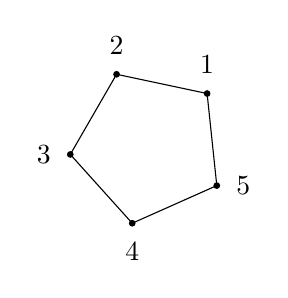
\begin{tikzpicture}%[color=DarkBlue]
\def\n{5}
\def\radius{1}
\def\rotation{-30}
\def\circrad{1pt}
\def\deg{360/\n}
\pgfmathsetmacro\nminusone{\n-1}

% \foreach \x in {1,...,\n}
% {
	\def\x{1}
	\pgfmathsetmacro\myangle{\x*\deg+\rotation};
	\filldraw (\myangle:\radius cm) circle (\circrad) node[label=$1$](a\x){};
	\def\x{2}
	\pgfmathsetmacro\myangle{\x*\deg+\rotation};
	\filldraw (\myangle:\radius cm) circle (\circrad) node[label=$2$](a\x){};
	\def\x{3}
	\pgfmathsetmacro\myangle{\x*\deg+\rotation};
	\filldraw (\myangle:\radius cm) circle (\circrad) node[label=left:$3$](a\x){};
	\def\x{4}
	\pgfmathsetmacro\myangle{\x*\deg+\rotation};
	\filldraw (\myangle:\radius cm) circle (\circrad) node[label=below:$4$](a\x){};
\def\x{5}
	\pgfmathsetmacro\myangle{\x*\deg+\rotation};
	\filldraw (\myangle:\radius cm) circle (\circrad) node[label=right:$5$](a\x){};


\foreach \y in {1,...,\n}
	{

	\pgfmathsetmacro\z{\y+1}
% 	{
		% \ifthenelse{\y < \n+1}
		% {
		\pgfmathsetmacro\myangley{\y*\deg+\rotation}
		\pgfmathsetmacro\myanglez{\z*\deg+\rotation}
		\draw (\myangley:\radius cm) -- (\myanglez:\radius cm);
% 		}{}

	}

\end{tikzpicture}
\end{center}
\caption{$C_5$, the cycle of length 5.} \label{fig:C5}
\end{marginfigure}

We also have $\alpha(C_5^2)\geq 5$, that is, you can send 5 different 2 symbol messages. These messages are: $\{(1,1),(2,3)(3,5),(4,2),(5,4)\}$, using the labelling of \cref{fig:C5}. 
In particular, $2<\sqrt{5} \leq \Theta(C_5)$, so our naive bound of $2$ is not optimal.

To prove an upper bound on $\Theta$, we'd like a function $
\theta(G)$ such that
\begin{enumerate}
	\item $\alpha(G) \leq \theta(G)$ \label{enum:theta1}
	\item $\theta(G\boxtimes H)\leq \theta(G) \theta(H)$.  \label{enum:theat2}
\end{enumerate}
Then, as in \cref{lem:chrom_num_shannon_capacity}, any such function will upper bound $\Theta$, i.e., $\Theta(G) \leq \theta(G)$. Ideally, $\theta(C_5)= \sqrt{5}$, to prove the lower bound of $\sqrt{5}$ is optimal. This would confirm that we've found a sharper upper bound than $\chi (\bar G)$.

One function satisfying all of these is the \defn{Lov\'asz theta}\sidenote{\cite{Lovasztheta}}, defined as follows.
Let $G$ be a graph with $V(G) = [n]$. A collection $v_1,v_2,\dotsc,v_n\in \R^d$ is an \defn{orthonormal representation} of $G$ if
\begin{itemize}
	\item $\|v_i\| = 1$,
	\item $v_i \perp v_j$ if $i$ and $j$ are not adjacent. 
\end{itemize}
\marginnote{Every graph has an orthonormal representation in dimension $n$.}
Let the \defn{value}[orthonormal representation!value] of an orthonormal representation be
\[
\min_{\|c\|=1} \max_{v_i} \frac{1}{\braket{v_i,c}^2}
\]
where $\braket{\cdot,\cdot}$ is the Euclidean inner product (dot product).
The vector $c$ acheiving the minimum is called a \emph{handle}.
Finally, define $\theta(G)$ as the minimal value over orthonormal representations.

That $\theta(G)$ satisfies points \labelcref{enum:theta1,enum:theat2} is the content of \cref{lem:alpha_less_than_theta,lem:shannon_cap_theta_submult}. That $\theta(C_5) \leq \sqrt{5}$ is the content of  \cref{lem:theta_C5}. This will conclude our discussion of Shannon capacity.

\begin{lemma} \label{lem:alpha_less_than_theta}
$\alpha(G)\leq \theta(G)$
\end{lemma}
\begin{proof}	
Let $v_1,\dotsc,v_n$ be the optimal orthonormal representation of $G$ with handle $c$. Let $\alpha(G) = k$, and suppose $\{1,2,\dotsc,k\}$ form an independent set. Then $v_1,\dotsc,v_k$ can be completed to an orthonormal basis, so
\[
	1=\|c\|^2 = \braket{c,c} \geq \sum_{i=1}^k (\braket{c,v_i})^2  \geq \frac{k}{\theta(G)}
\]
since
% \[
$\theta(G) \geq \frac{1}{\braket{c,v_i}^2}$.
 % \]
\end{proof}


\begin{lemma}\label{lem:shannon_cap_theta_submult}
\[
\theta(G\boxtimes H)\leq \theta(G)\theta(H).
\]
\end{lemma}
\begin{proof}	
Observation: if $u,v\in U$ and $x,y \in V$, then 
\[
\braket{u\otimes x, v \otimes y} = \braket{u,v}\braket{x,y}
\]
\marginnote{We can see this by working in components: if $u = (u_i)$, $v = (v_i)$, $x = (x_i)$, $y = (y_i)$, then $\braket{u\otimes x, v\otimes y} = \sum_{i,j} u_i x_j v_i y_j$ which we may regroup into the product of the two inner products.}

% \begin{remark}
If $u_1,\dotsc,u_n$ is an o.r. of $G$ with handle $c$, and $v_1,\dotsc,v_n$ is an o.r. of $H$ with handle $d$, then $(u_i\otimes v_j)$ is an o.r. of $G\boxtimes H$, by the above identity.

Let $c\otimes d$ be a handle. Then
\begin{align*}
\theta(G\otimes H) &\leq \max_{u_i,v_j}\frac{1}{ (\braket{c\otimes d, u_i\otimes v_j})^2}\\ &=\max_{u_i,v_j} \frac{1}{(\braket{c,u_i})^2 (\braket{d,v_j})^2}\leq \theta(G)\theta(H).
\end{align*}
% \end{remark}
\end{proof}

\begin{lemma} \label{lem:theta_C5}
$\theta(C_5)\leq\sqrt{5}$.
\end{lemma}
\begin{proof}	
Start with 
\begin{align*}	
v_{i+1} = \frac{(\cos( \tfrac{2\pi}{5}i),(\sin( \tfrac{2\pi}{5}i), p)}{\sqrt{1+p^2}}
\end{align*}
and increase $p$ from zero until each $v_i \perp v_{i+2},v_{i+3}$. 
\begin{figure*}[ht]
% \includegraphics[width=.25\linewidth]{graphics/C5p=0.pdf}\includegraphics[width=.25\linewidth]{graphics/C5p=p3.pdf}\includegraphics[width=.25\linewidth]{graphics/C5p=p6.pdf}\includegraphics[width=.25\linewidth]{graphics/C5p=p0.pdf}
\includegraphics[width=.33\linewidth]{graphics/C5p=0.pdf}\includegraphics[width=.33\linewidth]{graphics/C5p=p45.pdf}\includegraphics[width=.33\linewidth]{graphics/C5p=p0.pdf}
\caption{From left to right, the vectors $v_i$ with $p=0,0.45,\frac{1+\sqrt{5}}{4}\approx 0.89$. The intuition is that we are starting with our five vectors equally spaced on the unit circle. Then we ``close the umbrella'', increasing $p$, and pointing the vectors towards the $z$-axis, until each vector is orthogonal to the two vectors across from it.}
\end{figure*}

We have $(1,0,p) \perp (\cos \tfrac{4\pi}{5}, \sin \tfrac{4\pi}{5},p)$ if $-p^2 = \cos \tfrac{4\pi}{5}$. Then $p^2 = \frac{1+\sqrt{5}}{4}$. Now, we may check that at this value of $p$, each $v_i \perp v_{i+2},v_{i+3}$. That is, the $v_i$ form an orthonormal representation of $C_5$. Take $c = (0,0,1)$. Then $\braket{c,v_i} = \frac{p}{\sqrt{1+p^2}}$ for all $i$, and $\frac{1}{\big( \frac{p}{\sqrt{1+p^2}} \big)^2} = \dotsm = \sqrt{5}$.
\end{proof}